\section{Recerca genealògica}

    \paragraph{}
    El segon bloc d’eines que FamilySearch posa a disposició dels usuaris i aficionats a la genealogia són les eines necessàries per cercar en el seu immens catàleg de registres, col·leccions, genealogies i llibres genealògics.

    Existeixen diferents funcionalitats de cerca segons el tipus d'informació que es vol cercar. A continuació detallem la informació principal de cada una.

    \subsection{Cerca de registres}

        \paragraph{}
        La cerca de registres és sens dubte la principal funcionalitat de cerca que queda a disposició dels usuaris. Aquesta permet cercar avantpassats ja difunts en els registres històrics de FamilySearch.

        La cerca pot ser delimitada mitjançant diferents paràmetres de cerca i refinada posteriorment mitjançant l’ús de filtres. Els principals paràmetres amb els quals es pot configurar la cerca són:

        \begin{itemize}
            \item Nom i cognoms
            \item Cercar pel lloc i data aproximada o exacte d’esdeveniments particulars.
            \item Nom i cognoms dels relatius més propers com poden ser per exemple els pares o la parella.
            \item Restringir per localització del registre o persona. Pot ser una restricció de continent, país, província, ciutat, etcètera.
            \item Restringir per tipus de registre. Per exemple, obtenir només registres de naixement, baptisme, casament, servei militar, etcètera.
            \item Restringir per número de lot.
            \item Restringir per número de microfilm.
            \item Nivell d’exactitud desitjat sobre els camps introduïts. Es pot decidir entre un nivell més lax o un que intenti satisfer totes les condicions que han estat introduïdes.
            \item Restricció per col·lecció. Una col·lecció és una font de dades en concret. Per exemple, el cens de Nova York del 1905.
        \end{itemize}

        La figura~\ref{fig:fsSearcher} mostre el formulari de cerca bàsic.

        \begin{figure}[h]
            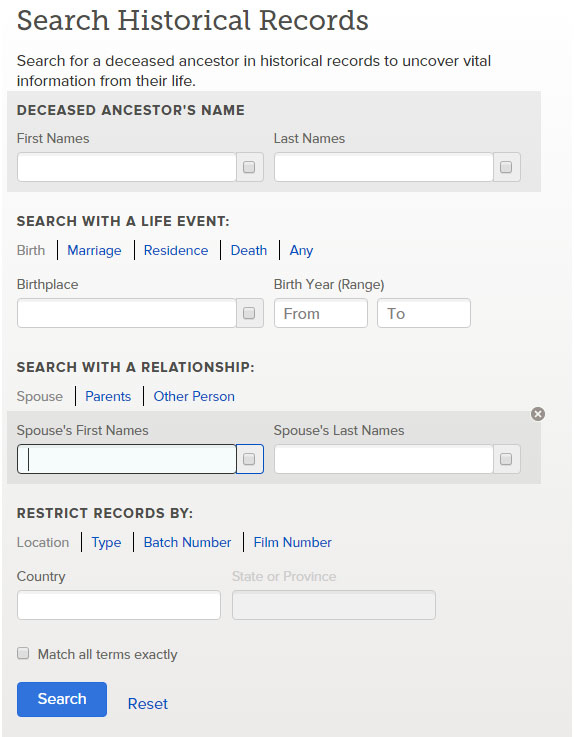
\includegraphics[scale=0.4]{03/searchForm}
            \centering
            \caption{Exemple del cercador de registres.\label{fig:fsSearcher}}
        \end{figure}


    \subsection{Cerca de genealogies}

        \paragraph{}
        La cerca de genealogies consisteix en la cerca sobre els arbres de família pujats i creats a FamilySearch per altres usuaris o provinents de registres oficials. La fiabilitat de les línies familiars creades per usuaris, varia d’arbre en arbre i els usuaris estan més que convidats a comprovar la veracitat de les genealogies resultants de la cerca.

        La cerca de genealogies es pot concretar mitjançant els següents paràmetres:

        \begin{itemize}
            \item Nom i cognoms
            \item Cercar pel lloc i data aproximada o exacte d’esdeveniments particulars.
            \item Nom i cognoms dels relatius més propers com poden ser els pares o la parella.
            \item Restringir els arbres genealògics retornats a aquells que han estat creats per usuaris o importats de diferents sistemes i arxius oficials.
        \end{itemize}


    \subsection{Cerca per catàleg}

        \paragraph{}
        Els catàlegs són materials genealògics com poden ser llibres, materials en línia, pel·lícules de microfilm, microfiche i altres publicacions, com per exemple, revistes. Molts d’aquests recursos poden ser agafats en préstec en els centres d’història de FamilySearch.


    \subsection{Cerca en llibres d'història genealògica}

        \paragraph{}
        La col·lecció de llibres d’història genealògica consisteix en més de 200.000 publicacions digitalitzades provinents de les més importants llibreries d’història familiar existents. La col·lecció inclou, evidentment, històries de família, revistes genealògiques, guies d’iniciació a la recerca genealògica, diccionaris geogràfics, històries medievals i arbres genealògics.


    \subsection{Wiki de FamilySearch}

        \paragraph{}
        La wiki de FamilySearch és una petita enciclopèdia que pretén assistir, sobretot als nou vinguts en el món de la recerca genealògica, a comprendre com conduir i enfocar la recerca depenent de les preguntes o informació que estiguin intentant respondre o trobar.

        De la wiki cal destacar la informació disponible per cada regió, país o província. Per cada un d'aquests nivells, es disposa d'informació sobre quins poden ser els punts o registres d’entrada més interessants segons la informació que s'estigui cercant.
